\bf{Example}

Let $ H=2, W=3, R=[0,1,1,0,0,1], C=[0,0,1,1,2,2], $ and $ Q=2. $ 

The grader first calls \t{give_initial_chart(2, 3, [0, 1, 1, 0, 0, 1], [0, 0, 1, 1, 2, 2]).} 

At first, the seating chart is as follows.

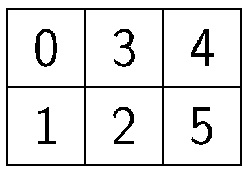
\includegraphics{image-000.jpg}

Let's say the grader calls \t{swap_seats(0, 5).} After the request 0, the seating chart is as follows

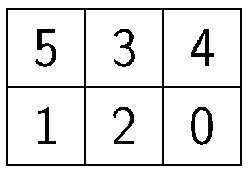
\includegraphics{image-001.jpg}

The sets of seats corresponding to the contestants $ \{0\}, \{0,1,2\}, $ and $ \{0,1,2,3,4,5\} $ are rectangular and beautiful. Thus, the beauty of this seating chart is $ 3, $ and \t{swap_seats} should return $ 3. $ 

Let's say the grader calls \t{swap_seats(}0, 5) again. After the request $ 1 $ , the seating chart goes back to the initial state. The sets of seats corresponding to the contestants $ \{0\}, \{0,1\}, \{0,1,2,3\} $ and $ \{0,1,2,3,4,5\} $ are rectangular and beautiful. Hence, the beauty of this seating chart is $ 4 $ , and \t{swap_seats }should return $ 4 $ .

The files \t{sample-01-in.txt} and \t{sample-01-out.txt} in the zipped attachment package correspond to this example. Other sample inputs/outputs are also available in the package.
